\testCom
{%Номер задачи
	3.198
}
{%Условие
	условие
}
{%Дано
	дано
}
{%Найти
	найти
}
{%Решение
	%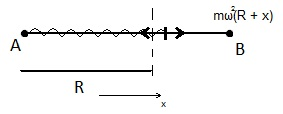
\includegraphics[height=30mm]{3_33.jpg}\\
	Для начала заметим, что $\avr{j(r)} = e^{-2 \gamma r} \avr{J_0}$\\
	$\left( \avr{\omega} = \avr{\rho \xi^2} = \frac{\avr{j}}{\upsilon} \right),$ а также можно ввести вектор (в нашем случае он будет скалярном) Умова для потерь энергии:\\
	$\langle \vec J_p \rangle = \langle \vec J_0 \rangle - \langle \vec J(\vec r) \rangle$, тогда \\
	потери энергии можно записать в виде\\
	$W = \int\limits_{t_1}^{t_2} \int\limits_{S(r)} \langle \vec J_p \rangle \, d\vec S = (t_2 - t_1) \int\limits_{S(r)} \langle \vec J_0 \rangle - \langle \vec J(r) \rangle \, d \vec S$\\
	$W = 4 \pi r^2 \avr{J_0} (1 - e^{-2 \gamma r}) t = 4 \pi r^2 \avr{J_0} (e^{2 \gamma r} - 1) t$\\
}

